\section{Introduction}

A key objective of present-day ecosystem ecology is to develop a predictive understanding of how terrestrial ecosystems will respond to rapid and widespread enviromental changes defining the Anthropocene. 
Plant functional traits serve as bellwethers of many aspects of plant ecophysiology, and understanding how traits respond to biotic and abiotic forcings has become a top priority in terrestrial ecology.
As I discussed in Chapter 1, global trait databases are useful for evaluating theories about plant ecological strategies and can be used to constrain parameters of dynamic vegetation models.

However, there are fundamental limits on the sorts of ecological questions that can be answered using static trait databases.
For one, such databases are spatially and phylogenetically incomplete, often in domains most critical to the global climate system such as boreal and tropical forests~\cite{jetz2016_diversity}.
More importantly, because these databases generally do not contain observations collected on the same individuals through time, they are limited in their ability to inform us about direct dynamic responses of plant function to environmental changes.
These changes are perhaps most pronounced in deciduous plants, whose leaves within a single season undergo a full life cycle accompanied by dramatic changes in pigment concentrations~\cite{yang_2016_seasonal}, morphology~\cite{poorter_2009_causes}, and productivity~\cite{parent_2010_modelling}.
Such intra-specific and intra-individual changes also occur in evergreen plants.
For instance, in tropical evergreen broadleaf trees, leaf biochemistry and productivity varies significantly with leaf and plant age~\cite{kitajima_1997_decline,Kitajima_2013_leaf,chavana_bryant_2016_leaf,wu_leaf_2016}.
Similarly, conifer needles undergo morphological and biochemical changes over the course of their lifetime that reflect shifting priorities in terms of ecological strategy~\cite{kuusk_2017_major}.
Besides these developmental changes, plant traits also respond to biotic and abiotic stressors, including
drought~\cite{sun_2018_reflectance,buchner_2017_drought,bayat_2016_remote},
heat~\cite{chapin_1996_physiological,serbin_2012_spectroscopic},
elevated CO$_2$~\cite{medlyn_using_2015,lindroth_2010_impacts},
insect infestation~\cite{divittorio_2009_spectral,marti_2012_metabolomics},
and pathogens~\cite{horst_2009_ustilago}.

Understanding the contributions of these many different drivers of plant trait variability necessarily requires large sample sizes over a wide range of conditions.
Meanwhile, observing responses directly requires measurements through time.
Traditional methods for assessing traits are ill-suited to this task because they are generally labor intensive and often require destructive sampling.
As I discussed in Chapter 2, spectral measurements of plant tissues are capable of providing a fast and non-destructive assessment of plant traits.
Leaf reflectance spectra have been widely used to study plant functional traits,
both to elucidate patterns of natural variability~\cite{cavenderbares_2017_harnessing,asner_2015_quantifying}
and for assessing trait responses to stress~\cite{serbin_spectroscopic_2014,bayat_2016_remote,sun_2018_reflectance}.
Furthermore, by clarifying the relationships between plant optical properties and traits, studies using leaf spectra are essential to the remote mapping and monitoring of traits~\cite{schneider2017_mapping,schimel2013_observing,schimel2015_observing,jetz2016_diversity}.

Although, a variety of traits have been estimated empirically from spectra, the contribution of those traits to actual reflectance is not always clear.
Some of the traits estimated empirically, such as $V_{c,\max}$ and $J_{c,\max}$, are not actually properties of plants but rather model parameters inferred from measurements of plant activity, so they by definition cannot influence plant reflectance.
Similarly, elemental concentrations and ratios (particularly leaf N) are among the most common targets of spectroscopy, but these elements are present in plants primarily in larger molecules.
However, the fact that these ``invisible'' traits can be accurately estimated from spectra indicates that they are often correlated related to other actually ``visible'' traits, but the exact nature of these correlations is still not well understood.
In this study, I focus on six foliar traits (hereafter known as ``optical'' traits) that do contribute directly to leaf reflectance, and which are themselves relevant to plant function (Figure~\ref{fig:prospect_coefficients}):
(1) Leaf mesophyll structure, expressed as the effective number of leaf mesophyll layers, provides a physical mechanism for leaf adaptation to light independent of biochemical changes in photosynthetic machinery~\cite{ivanov_2016_photosynthesis,schollert_2017_leaf}.
(2) Leaf chlorophyll content (the sum of chlorophyll $a$ and $b$) drives the amount of photosynthetically active radiation absorbed by leaves and is therefore closely related to plant photosynthesis~\cite{croft_2017_chlorophyll}.
Chlorophyll absorbs strongly in the visible range, particularly in the blue and red regions, where absorbance is $>$90\%.
(3) Leaf carotenoid pigments are related to the xanthophyll cycle, a key mechanism for preventing plant photooxidiative stress under drought, heat stress, and high light~\cite{ruban_2007_identifcation}.
Carotenoid pigments absorb light most strongly in blue, to a lesser extent, green wavelengths.
(4) Leaf anthocyanin pigments have a somewhat poorly understood role in plant physiology, but generally seem to enhance leaf tolerance to a wide range of stressors including drought, ultraviolet radiation, heavy metals, and photooxidation~\cite{gould_2004_nature}.
Anthocyanins absorb most strongly in green and, to a lesser extent, blue wavelengths.
(5) Leaf water content is closely related to leaf health and productivity, and is useful as an indicator of overall plant water status~\cite{penuelas_1994_reflectance,kramer_1995_water,cheng_2011_spectroscopic,chavana_bryant_2016_leaf}.
Water is the mean factor driving leaf absorbance in shortwave infrared wavelengths ($>$1300 nm), and has particularly deep absorption features around 1450, 1950, and 2500 nm.
(6) Finally, leaf dry mass per area is indicative of a wide variety of plant functional characteristics~\cite{poorter_2009_causes} and is a key parameter in determining plant ecological strategy~\cite{wright_worldwide_2004,reich_world-wide_2014}.
Although exact molecular composition varies substantially across species and individuals, leaf dry mass is generally dominated by minerals, organic acids, structural and nonstructural carbohydrates, phenolics, proteins, lignin, and lipids~\cite{poorter_2009_causes}.
Collectively, these molecules have an absorption peak in very blue wavelengths, negligible absorption in the visible and near-infrared, and gradually increasing absorption across the shortwave infrared region.

\begin{figure}
  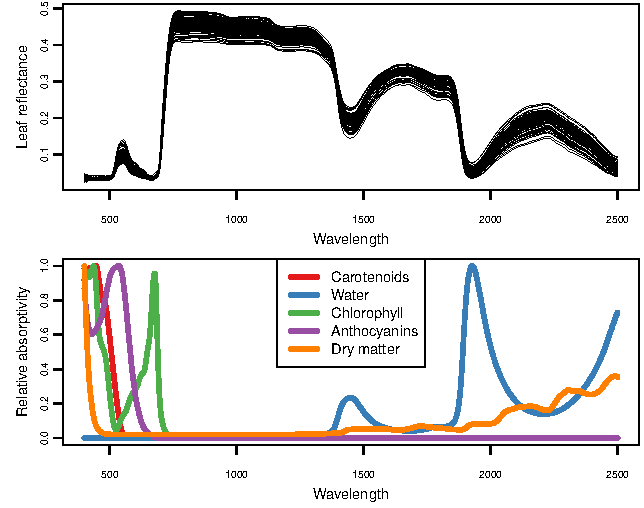
\includegraphics[width=\textwidth]{{figures/sigspec2-1}.pdf}
  \caption{\
    (Top) Example reflectance spectra of \textit{Acer rubrum} leaves.
    (Bottom) Normalized absorption coefficients for optical traits in this study.
  }\label{fig:prospect_coefficients}
\end{figure}

The six traits described above are used by the PROSPECT leaf radiative transfer model to simulate leaf reflectance and transmittance~\cite{jacquemoud_1990_prospect,feret_2008_prospect,feret_2017_prospectd}.
PROSPECT has been used extensively for the simulation of leaf and, (combined with canopy models) canopy reflectance, as well as for estimation of leaf spectral characteristics through spectral inversion~\cite[Chapter 2,][]{jacquemoud_2009_prosail}.
Unlike empirical approaches for estimating leaf properties from spectra, including spectral indices~\cite{lemaire_2004_towards,feret_2011_optimizing} and partial least squares regression (PLSR)~\cite{serbin_2011_leaf}, PROSPECT aims to provide a causal understanding of leaf optical properties.
This means that, by design, PROSPECT intends to be generic across all species and conditions, and, more importantly, makes it a useful tool for applications where the links between leaf properties and spectra are important, such as modeling leaf absorbance for photosynthesis and for improving representations of energy balance in terrestrial biosphere models.
However, the extent of PROSPECT's generality has not been well tested, with most PROSPECT studies focusing on a relatively small set of species that are fairly similar to those used for PROSPECT's original calibration~\cite{feret_2008_prospect,feret_2011_optimizing,feret_2017_prospectd,li_2011_retrieval,wang_2015_leaf}.

The above discussion culminates in the following three questions:
First, how well can leaf optical traits be estimated from PROSPECT inversion over a wide range of species and experimental designs?
Second, how do leaf optical traits vary across a variety of environmental conditions and species?
Specifically, how is intraspecific variability in optical traits related to various growing conditions including local climate, canopy light environment, and exposure to pathogens?
As well, how well can interspecific variability in traits be explained by species attributes frequently used for grouping species into functional types (e.g. plant growth form, photosynthetic pathway, phenological habit)? 
Third, how are leaf optical traits related to other leaf traits not directly estimable from PROSPECT inversion?
To address these questions, I applied my PROSPECT inversion methodology (Chapter 2) to a large database of leaf spectra and traits collected in a variety of natural and experimental settings.
